\documentclass[a4paper,12pt]{article}
   % Packages and definitions:
   % {
      \usepackage{float}
      \usepackage[english]{babel}
      \usepackage[utf8]{inputenc}
      \usepackage{amsmath}
      \usepackage{amssymb}
      \usepackage{color}
      \usepackage{subcaption}
      \usepackage{booktabs}
      \usepackage{tikz}
      \usepackage{multirow}
      \usetikzlibrary{decorations.pathreplacing}
      \usepackage{graphicx,epstopdf}
      \usepackage{cleveref}
      \usepackage{collcell} % loads array
      \usepackage{listings}
      \newcolumntype{m}{>{$} r <{$}}
      \newcolumntype{u}{>{$[\collectcell\si} l <{\endcollectcell]$}}
      \newcommand{\approxtext}[1]{\ensuremath{\stackrel{\text{#1}}{=}}}
      \newcommand{\matr}[1]{\mathbf{#1}}
      \newcommand{\partt}[2]{\ensuremath{\dfrac{\d {#1}}{\partial {#2}}}}
      \renewcommand{\d}[1]{\ensuremath{\operatorname{d}\!{#1}}} % non-italized differentials
      \newcommand{\h}[0]{\ensuremath{\hbar}} % hbar
      \newcommand{\qed}[0]{\ensuremath{\tag*{$\square$}}} % QED square
      \def\changemargin#1#2{\list{}{\rightmargin#2\leftmargin#1}\item[]}
      \let\endchangemargin=\endlist 
      \usepackage{amsthm}
      \theoremstyle{plain}
      \newtheorem{thm}{theorem} % reset theorem numbering for each chapter
      \theoremstyle{definition}
      \newtheorem{defn}[thm]{definition} % definition numbers are dependent on theorem numbers
      \newtheorem{exmp}[thm]{example} % same for example numbers
      \bibliographystyle{natbib}
      \renewcommand{\theequation}{\thesection.\arabic{equation}}
      \newcommand{\ts}{\textsuperscript} 

      \definecolor{dkgreen}{rgb}{0,0.6,0}
      \definecolor{gray}{rgb}{0.5,0.5,0.5}
      \definecolor{mauve}{rgb}{0.58,0,0.82}

      \lstset{frame=tb,
        language=Java,
        aboveskip=3mm,
        belowskip=3mm,
        showstringspaces=false,
        columns=flexible,
        basicstyle={\small\ttfamily},
        numbers=none,
        numberstyle=\tiny\color{gray},
        keywordstyle=\color{blue},
        commentstyle=\color{dkgreen},
        stringstyle=\color{mauve},
        breaklines=true,
        breakatwhitespace=true,
        tabsize=3
      }
% }
\title
{
	\textbf
	{
      Computer assignment 1: \\
      Depletion forces
   }
}

\author{Henrik Åhl}
\date{\today}

\begin{document}
\begin{titlepage}
	
   \maketitle 
	\begin{center}
		\phantom{a}
		{Department of Astronomy and Theoretical Physics, Lund University}
		\\[2cm]
		{Project supervised by Anna Bille}
		\vfill
		\includegraphics[height=4cm]{logocLUeng.pdf}
	\end{center}
	\thispagestyle{empty} % do not count pages just yet
\end{titlepage}
\section{Introduction}
   The concept of depletion forces is an example of how abstract theoretical modelling
   can be used to explain direct physical behaviour on a nanometer scale. It does so by 
   adopting the concept of entropy and entropic forces, and applies them into a biological
   context -- namely in the context of dilute solutions. Although the context is
   not completely necessary for the conclusions to hold, it holds high
   historical significance, and can particularly be used to explain how larger molecules
   submerged in a dilute solution can be affected by smaller molecules through forces 
   occuring when the so called \textit{depletion zones} of the larger
   molecules overlap. In a practical context the concept can also be used to explain even 
   parts of the so scientifically distant procedure of wine purification, where the concept is 
   utilized in order to filter unwanted particles from the wine itself.~\cite{wine}.
   
   The depletions zones that are modellized do in essence construct the space where the
   center of the smaller molecules (in an ideal, symmetrical model) can't reach, and make 
   up the basis for how attractive forces can arise due a greater volume being
   accessible to the smaller particles, thereby shifting the states of maximal
   entropy.~\cite{lecnotes}

\section{Modelling depletion forces}
   Maximizing entropy can be said to be equivalent to minimizing the
   \textit{free energy} in a system. In a system with $N$ small balls (smaller
   molecules) of radius $r$, and one larger ball (larger molecule) of radius
   $R$, in a cavity of some shape. The cavity can then be
   imagined to be surrounded by a shell of thickness $r$ through which the
   center of the other balls cannot reach. As a consequence, when the surface of the
   large molecule comes into a distance of $D<2r$ from the boundary, the
   depletion zones will overlap, causing an effective entropic force to act upon
   the system, driving the molecule towards the boundary. Additionally, the
   effect will likewise cause an attraction between larger objects in general
   within the system, so that \emph{two} larger molecules similarily would be
   driven together. 
   
   The probability density for a given microstate in our system can be written
   as 

   \begin{align}
      \rho_N(\mathbf r_1, \ldots, \mathbf r_N) = \frac{e^{-\beta U(\mathbf r_1,
      \ldots, \mathbf r_N)}}{Q}
   \end{align}

   where $Q$ is the partition function. This implies that the average force on a
   particle at position $\mathbf r_1$ can be described by the negative gradient
   \begin{align}
      \mathbf{f} (\mathbf{r}_1) \equiv \left\langle \nabla_1 U \right\rangle = -
      \frac{\int \d{ \mathbf{r}_2} \ldots \d{ \mathbf{r}_N} 
      \left( \nabla_1 U \right) 
      e^{ -\beta U( \mathbf{r}_1, \ldots, \mathbf{r}_N)}}
      {\int \d{ \mathbf{r}_2} \ldots \d{ \mathbf{r}_N} e^{-\beta U( \mathbf{r}_1,
      \ldots, \mathbf{r}_N)}}
      \label{eq:potofmeanforce}
   \end{align}

   as a direct effect of the definition. This must in turn be equivalent to
   stating that

   \begin{align}
      \mathbf f(\mathbf r_1) = kT\nabla_1 \ln \rho(\mathbf r_1).
      \label{eq:exercise_1}
   \end{align}
   
   This we know since $\nabla_1 \ln\rho(\mathbf{r_1})$ can trivially be rewritten
   as $\frac{\nabla_1\rho(\mathbf r_1)}{\rho(\mathbf r_1)}$, which would
   render the exact same result as in \cref{eq:potofmeanforce} once we realize that we have
   to multiply by a factor $\beta^{-1}$ to achieve identity, since $Q$ is nothing
   but a constant and will not be affected by the differentiation. 
  
   To establish how the free energy in our system then depends on the position
   of the big molecule, we can through various assumptions assert the following: 

   \begin{align}
      D &\equiv R_s - R - r_0 \\
      f(D) &\approx -\frac{\partial F}{\partial D} = ckT \frac{\partial
      V}{\partial D} \label{eq:dep_force} 
   \end{align}

   Here $F$ is the free energy of the system whereas $D$ is a constant describing 
   the distance between the big ball and the center of the cavity, made up of the 
   constants for the radius of the cavity
   (assumedly spherical) $R_s$, the radius of the ball, $R$, and the distance
   between the \emph{center} of the ball and the center of the cavity,
   $r_0$. $c = N/V$ in turn acts as a parameter for the concentration of small balls within the
   system. $V$ describes the volume of the cavity, and is here
   assumed to be roughly the same as the volume that is available to the smaller balls.

   For a flat boundary, i.e. a box rather than a sphere as a cavity, the area of
   where the depletion zones of the big ball and the boundary meet can be given
   by

   \begin{align}
      \frac{\partial V_{ov}}{\partial D} = -A(D)
   \end{align}
   
   where $V_{ov}$ is the overlapping volume. 

   From figure 2 in the lecture provided (see \cite{lecnotes}), we can therefore establish that
   the distance $h$, between the area $A$ and the boundary of the ball, as well
   as the auxillary distance $\alpha$, between the center of the ball and $A$ can be described as 

   \begin{align*}
      h &= 2r - D \\
      \alpha &= R - r - D.
   \end{align*}
   
   It follows that

   \begin{align}
      \alpha^2 + a^2 = (R + r)^2 \Leftrightarrow a^2 = 4rR + 2(r-R)D - D^2
   \end{align}

   from pure trigonometrics, which gives us the sought-after area $A$. Inserted 
   into \cref{eq:dep_force} we then get that

   \begin{align}
      f(D) = -ckT\pi \left[ 4rR + 2(r-R)D - D^2 \right] 
   \end{align}
   when $D \in [0, 2r]$, and otherwise 0. Assuming further that $F(2r) = 0$ is a
   boundary condition, integrating for the free energy renders

   \begin{align}
      F(D) &= \int_D^{2r} f(D') \d D' = ckT\pi\left[ 4rRD' + (r-R)D'^2 
      \right]_D^{2r} \nonumber \\
      &= ckT\pi\left[ 8r^2R + 4(r^3-r^2R) - \frac{8}{3}r^3 - 4rRD
      - (r-R) D^2 + \frac{D^3}{3}\right] \nonumber \\
      &= ckT\pi\left[ 4r^2R +
      \frac{4}{3}r^3 - 4rRD - rD^2 + RD^2 + \frac{D^3}{3}\right] \nonumber \\
      &= -ckT\pi(2r-D)\left[
      2r\left( R +\frac{r}{3} \right) - D\left( R - \frac{r}{3}\right) -
      \frac{D^2}{3} 
      \right]
      \label{eq:free_en}
   \end{align}
   
   as a final expression.

   In a spherical cavity however, the area of interest is instead given by
   $A = 2\pi h(D)(R_s - r)$. In this case one can from geometric analysis
   establish that 

   \begin{align*}
      (R + r)^2- (R_s -r)^2 &= (R -r +D - h)^2 - (R_s -r - h)^2 \Leftrightarrow \\
      0 &= 4Rr - D^2 - 2RD + 2Rh + 2rD + 2Dh - 2R_sh \Leftrightarrow \\
      h &= \frac{D^2 + 2RD - 2rD - 4R}{2(R + D - R_s)}.
   \end{align*}

   When then factorized and inserted into \cref{eq:dep_force}, the force is
   given by 
   \begin{align}
   f(D) = -ckT\pi \frac{(2r-D)(2R+D)(R_s-r)}{R_s - R - D}
      \label{eq:force_spherical_cav}
   \end{align}
   
   whereas correspondingly, the free energy is given through integrating. By
   first doing a polynomial long division, it can be noted that our expression
   within the brackets can be rewritten as 
   \begin{align*}
      D - (2r-R-R_s) + \frac{2rR + 2rR_s + R^2-R_s^2}{R_s - R - D}.
   \end{align*}

   Integrating this with respect to $D$ simply results in 

   \begin{align*}
       -2r^2 + 2rR + 2rR_s - \frac{D^2}{2} + D(2r-R-R_s)~+ \\
      +~(2r-R_s+R)(R_s + R) \frac{\ln(R_s-R-D)}{\ln(R_s-R-2r)}
   \end{align*}
   which can be factorized into something that, when accounting for our
   prefactors in the free energy expressions, results in 

   \begin{align}
      F(D) = -ckT\pi (R_s-r)\left[ (2r-D)\left( R_s+R-r +
      \frac{D}{2}\right)\right.~+ \nonumber \\ 
      +~(2r-R_s+R)(R_s+R)\ln(\ldots)\bigg].
      \label{eq:free_en_spherical}
   \end{align}
   
   Notably, the logarithm is of the form 
   \begin{align*}
      \ln\frac{R_s + d}{R_s + c} = \ln\frac{1 + \frac{d}{R_s}}{1 +
      \frac{c}{R_s}} = \ln(\ldots) - \ln(\ldots)
   \end{align*}
   that is ideal for Taylor expanding in ${R_s}^{-1}$. When doing so, we see
   that the logaritmic expressions simplify to 

   \begin{align*}
      \ln(\ldots) - \ln(\ldots) &= \frac{1}{R_s}(2r-D) +
      \frac{1}{2R_s^2}(2r-D)(2r+2R+D) + \\ &+\frac{1}{R_s^3}(2r-D)(4r^2 + 2Dr + 6Rr +
      D^2 + 3RD + 3R^2)
   \end{align*}

   where insertion into what we have, while letting $R_s$ tend towards infinity, 
   reveals that this energy too acts as the free energy for the flat boundary.

\section{Results}
   
   When running the simulation with the standard values, the results produced in
   \cref{fig:pmfa} appear. Notably, both trend lines correspond somewhat
   accurately to data, even though the trend line with $V_big$ omitted does not
   so as much as the one where it is not. Also, it is clearly seen that the
   limits for the simulation span between a length of 14--18 length units. This
   clearly corresponds to the identity $D = R_s - R - 2r$, as the values
   here are set to 30, 12 and 2 correspondingly, so that the depletion zones go
   from not overlapping at all, to overlapping completely. When the zones start
   overlapping, the free energy increases, since more volume is then available
   to the smaller spheres. During all simulations, if nothing else is noted, the
   amount of small balls round up to 50 specimen. 
  
   \begin{figure}[H]
      \centering
      \resizebox{.6\columnwidth}{!}{% GNUPLOT: LaTeX picture with Postscript
\begingroup
  \makeatletter
  \providecommand\color[2][]{%
    \GenericError{(gnuplot) \space\space\space\@spaces}{%
      Package color not loaded in conjunction with
      terminal option `colourtext'%
    }{See the gnuplot documentation for explanation.%
    }{Either use 'blacktext' in gnuplot or load the package
      color.sty in LaTeX.}%
    \renewcommand\color[2][]{}%
  }%
  \providecommand\includegraphics[2][]{%
    \GenericError{(gnuplot) \space\space\space\@spaces}{%
      Package graphicx or graphics not loaded%
    }{See the gnuplot documentation for explanation.%
    }{The gnuplot epslatex terminal needs graphicx.sty or graphics.sty.}%
    \renewcommand\includegraphics[2][]{}%
  }%
  \providecommand\rotatebox[2]{#2}%
  \@ifundefined{ifGPcolor}{%
    \newif\ifGPcolor
    \GPcolortrue
  }{}%
  \@ifundefined{ifGPblacktext}{%
    \newif\ifGPblacktext
    \GPblacktexttrue
  }{}%
  % define a \g@addto@macro without @ in the name:
  \let\gplgaddtomacro\g@addto@macro
  % define empty templates for all commands taking text:
  \gdef\gplbacktext{}%
  \gdef\gplfronttext{}%
  \makeatother
  \ifGPblacktext
    % no textcolor at all
    \def\colorrgb#1{}%
    \def\colorgray#1{}%
  \else
    % gray or color?
    \ifGPcolor
      \def\colorrgb#1{\color[rgb]{#1}}%
      \def\colorgray#1{\color[gray]{#1}}%
      \expandafter\def\csname LTw\endcsname{\color{white}}%
      \expandafter\def\csname LTb\endcsname{\color{black}}%
      \expandafter\def\csname LTa\endcsname{\color{black}}%
      \expandafter\def\csname LT0\endcsname{\color[rgb]{1,0,0}}%
      \expandafter\def\csname LT1\endcsname{\color[rgb]{0,1,0}}%
      \expandafter\def\csname LT2\endcsname{\color[rgb]{0,0,1}}%
      \expandafter\def\csname LT3\endcsname{\color[rgb]{1,0,1}}%
      \expandafter\def\csname LT4\endcsname{\color[rgb]{0,1,1}}%
      \expandafter\def\csname LT5\endcsname{\color[rgb]{1,1,0}}%
      \expandafter\def\csname LT6\endcsname{\color[rgb]{0,0,0}}%
      \expandafter\def\csname LT7\endcsname{\color[rgb]{1,0.3,0}}%
      \expandafter\def\csname LT8\endcsname{\color[rgb]{0.5,0.5,0.5}}%
    \else
      % gray
      \def\colorrgb#1{\color{black}}%
      \def\colorgray#1{\color[gray]{#1}}%
      \expandafter\def\csname LTw\endcsname{\color{white}}%
      \expandafter\def\csname LTb\endcsname{\color{black}}%
      \expandafter\def\csname LTa\endcsname{\color{black}}%
      \expandafter\def\csname LT0\endcsname{\color{black}}%
      \expandafter\def\csname LT1\endcsname{\color{black}}%
      \expandafter\def\csname LT2\endcsname{\color{black}}%
      \expandafter\def\csname LT3\endcsname{\color{black}}%
      \expandafter\def\csname LT4\endcsname{\color{black}}%
      \expandafter\def\csname LT5\endcsname{\color{black}}%
      \expandafter\def\csname LT6\endcsname{\color{black}}%
      \expandafter\def\csname LT7\endcsname{\color{black}}%
      \expandafter\def\csname LT8\endcsname{\color{black}}%
    \fi
  \fi
  \setlength{\unitlength}{0.0500bp}%
  \begin{picture}(7200.00,5040.00)%
    \gplgaddtomacro\gplbacktext{%
      \colorrgb{0.42,0.42,0.42}%
      \put(946,704){\makebox(0,0)[r]{\strut{}-4.9}}%
      \colorrgb{0.42,0.42,0.42}%
      \put(946,1213){\makebox(0,0)[r]{\strut{}-4.8}}%
      \colorrgb{0.42,0.42,0.42}%
      \put(946,1722){\makebox(0,0)[r]{\strut{}-4.7}}%
      \colorrgb{0.42,0.42,0.42}%
      \put(946,2231){\makebox(0,0)[r]{\strut{}-4.6}}%
      \colorrgb{0.42,0.42,0.42}%
      \put(946,2739){\makebox(0,0)[r]{\strut{}-4.5}}%
      \colorrgb{0.42,0.42,0.42}%
      \put(946,3248){\makebox(0,0)[r]{\strut{}-4.4}}%
      \colorrgb{0.42,0.42,0.42}%
      \put(946,3757){\makebox(0,0)[r]{\strut{}-4.3}}%
      \colorrgb{0.42,0.42,0.42}%
      \put(946,4266){\makebox(0,0)[r]{\strut{}-4.2}}%
      \colorrgb{0.42,0.42,0.42}%
      \put(946,4775){\makebox(0,0)[r]{\strut{}-4.1}}%
      \colorrgb{0.42,0.42,0.42}%
      \put(1651,484){\makebox(0,0){\strut{} 14}}%
      \colorrgb{0.42,0.42,0.42}%
      \put(2796,484){\makebox(0,0){\strut{} 15}}%
      \colorrgb{0.42,0.42,0.42}%
      \put(3941,484){\makebox(0,0){\strut{} 16}}%
      \colorrgb{0.42,0.42,0.42}%
      \put(5086,484){\makebox(0,0){\strut{} 17}}%
      \colorrgb{0.42,0.42,0.42}%
      \put(6231,484){\makebox(0,0){\strut{} 18}}%
      \colorrgb{0.42,0.42,0.42}%
      \put(176,2739){\rotatebox{-270}{\makebox(0,0){\strut{}$-ln(H(r))+ln(r^2)$}}}%
      \colorrgb{0.42,0.42,0.42}%
      \put(3940,154){\makebox(0,0){\strut{}$r$}}%
      \colorrgb{0.42,0.42,0.42}%
      \put(3940,4665){\makebox(0,0){\strut{}}}%
    }%
    \gplgaddtomacro\gplfronttext{%
      \csname LTb\endcsname%
      \put(5804,4602){\makebox(0,0)[r]{\strut{}Simulation results}}%
      \csname LTb\endcsname%
      \put(5804,4382){\makebox(0,0)[r]{\strut{}$V_{big}$ omitted}}%
      \csname LTb\endcsname%
      \put(5804,4162){\makebox(0,0)[r]{\strut{}$V_{big}$ not omitted}}%
    }%
    \gplbacktext
    \put(0,0){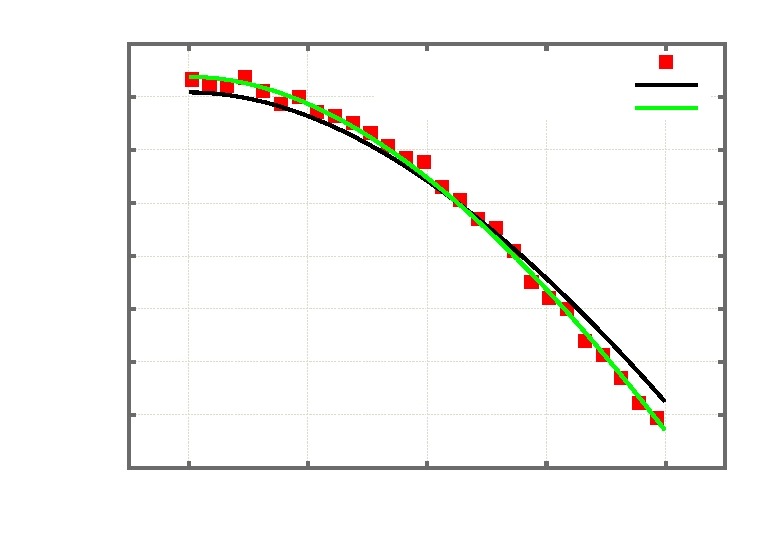
\includegraphics{pmfa}}%
    \gplfronttext
  \end{picture}%
\endgroup
}
      \caption{Simulation of depletion zone overlap effect on the free energy in
         a 3-dimensional cavity of spherical shape. Note that the y-axis is
         a similarity function that behaves like the free energy, but is not equal to
         it. Here it acts as a relational measure.}
      \label{fig:pmfa}            
   \end{figure}

   When the parameters are shifted somewhat however, this stability that is
   found in \cref{fig:pmfa} is lacking, both in \cref{fig:4xballs} and
   \cref{fig:gigaball}. The system notably starts oscillating extensively
   whenever depletion zones overlap, whereas our approximation of ommiting
   $V_{big}$ breaks down as well, particularly in the case of a bigger
   macromolecule. The fluctuations are a cause of the instability inherent to
   the dynamics of the system, occuring for example when many balls form
   structures next to each other. 

   \begin{figure}[H]
      \vspace*{1cm}
      \hspace*{-2cm}
      \centering
      \begin{minipage}[t]{.6\textwidth}		
         \vspace{0pt}
         \centering
         \resizebox{\columnwidth}{!}{% GNUPLOT: LaTeX picture with Postscript
\begingroup
  \makeatletter
  \providecommand\color[2][]{%
    \GenericError{(gnuplot) \space\space\space\@spaces}{%
      Package color not loaded in conjunction with
      terminal option `colourtext'%
    }{See the gnuplot documentation for explanation.%
    }{Either use 'blacktext' in gnuplot or load the package
      color.sty in LaTeX.}%
    \renewcommand\color[2][]{}%
  }%
  \providecommand\includegraphics[2][]{%
    \GenericError{(gnuplot) \space\space\space\@spaces}{%
      Package graphicx or graphics not loaded%
    }{See the gnuplot documentation for explanation.%
    }{The gnuplot epslatex terminal needs graphicx.sty or graphics.sty.}%
    \renewcommand\includegraphics[2][]{}%
  }%
  \providecommand\rotatebox[2]{#2}%
  \@ifundefined{ifGPcolor}{%
    \newif\ifGPcolor
    \GPcolortrue
  }{}%
  \@ifundefined{ifGPblacktext}{%
    \newif\ifGPblacktext
    \GPblacktexttrue
  }{}%
  % define a \g@addto@macro without @ in the name:
  \let\gplgaddtomacro\g@addto@macro
  % define empty templates for all commands taking text:
  \gdef\gplbacktext{}%
  \gdef\gplfronttext{}%
  \makeatother
  \ifGPblacktext
    % no textcolor at all
    \def\colorrgb#1{}%
    \def\colorgray#1{}%
  \else
    % gray or color?
    \ifGPcolor
      \def\colorrgb#1{\color[rgb]{#1}}%
      \def\colorgray#1{\color[gray]{#1}}%
      \expandafter\def\csname LTw\endcsname{\color{white}}%
      \expandafter\def\csname LTb\endcsname{\color{black}}%
      \expandafter\def\csname LTa\endcsname{\color{black}}%
      \expandafter\def\csname LT0\endcsname{\color[rgb]{1,0,0}}%
      \expandafter\def\csname LT1\endcsname{\color[rgb]{0,1,0}}%
      \expandafter\def\csname LT2\endcsname{\color[rgb]{0,0,1}}%
      \expandafter\def\csname LT3\endcsname{\color[rgb]{1,0,1}}%
      \expandafter\def\csname LT4\endcsname{\color[rgb]{0,1,1}}%
      \expandafter\def\csname LT5\endcsname{\color[rgb]{1,1,0}}%
      \expandafter\def\csname LT6\endcsname{\color[rgb]{0,0,0}}%
      \expandafter\def\csname LT7\endcsname{\color[rgb]{1,0.3,0}}%
      \expandafter\def\csname LT8\endcsname{\color[rgb]{0.5,0.5,0.5}}%
    \else
      % gray
      \def\colorrgb#1{\color{black}}%
      \def\colorgray#1{\color[gray]{#1}}%
      \expandafter\def\csname LTw\endcsname{\color{white}}%
      \expandafter\def\csname LTb\endcsname{\color{black}}%
      \expandafter\def\csname LTa\endcsname{\color{black}}%
      \expandafter\def\csname LT0\endcsname{\color{black}}%
      \expandafter\def\csname LT1\endcsname{\color{black}}%
      \expandafter\def\csname LT2\endcsname{\color{black}}%
      \expandafter\def\csname LT3\endcsname{\color{black}}%
      \expandafter\def\csname LT4\endcsname{\color{black}}%
      \expandafter\def\csname LT5\endcsname{\color{black}}%
      \expandafter\def\csname LT6\endcsname{\color{black}}%
      \expandafter\def\csname LT7\endcsname{\color{black}}%
      \expandafter\def\csname LT8\endcsname{\color{black}}%
    \fi
  \fi
  \setlength{\unitlength}{0.0500bp}%
  \begin{picture}(7200.00,5040.00)%
    \gplgaddtomacro\gplbacktext{%
      \colorrgb{0.42,0.42,0.42}%
      \put(946,704){\makebox(0,0)[r]{\strut{}-6}}%
      \colorrgb{0.42,0.42,0.42}%
      \put(946,1383){\makebox(0,0)[r]{\strut{}-5.5}}%
      \colorrgb{0.42,0.42,0.42}%
      \put(946,2061){\makebox(0,0)[r]{\strut{}-5}}%
      \colorrgb{0.42,0.42,0.42}%
      \put(946,2740){\makebox(0,0)[r]{\strut{}-4.5}}%
      \colorrgb{0.42,0.42,0.42}%
      \put(946,3418){\makebox(0,0)[r]{\strut{}-4}}%
      \colorrgb{0.42,0.42,0.42}%
      \put(946,4097){\makebox(0,0)[r]{\strut{}-3.5}}%
      \colorrgb{0.42,0.42,0.42}%
      \put(946,4775){\makebox(0,0)[r]{\strut{}-3}}%
      \colorrgb{0.42,0.42,0.42}%
      \put(1078,484){\makebox(0,0){\strut{} 14}}%
      \colorrgb{0.42,0.42,0.42}%
      \put(1794,484){\makebox(0,0){\strut{} 14.5}}%
      \colorrgb{0.42,0.42,0.42}%
      \put(2509,484){\makebox(0,0){\strut{} 15}}%
      \colorrgb{0.42,0.42,0.42}%
      \put(3225,484){\makebox(0,0){\strut{} 15.5}}%
      \colorrgb{0.42,0.42,0.42}%
      \put(3941,484){\makebox(0,0){\strut{} 16}}%
      \colorrgb{0.42,0.42,0.42}%
      \put(4656,484){\makebox(0,0){\strut{} 16.5}}%
      \colorrgb{0.42,0.42,0.42}%
      \put(5372,484){\makebox(0,0){\strut{} 17}}%
      \colorrgb{0.42,0.42,0.42}%
      \put(6087,484){\makebox(0,0){\strut{} 17.5}}%
      \colorrgb{0.42,0.42,0.42}%
      \put(6803,484){\makebox(0,0){\strut{} 18}}%
      \colorrgb{0.42,0.42,0.42}%
      \put(176,2739){\rotatebox{-270}{\makebox(0,0){\strut{}$-ln(H(r))+ln(r^2)$}}}%
      \colorrgb{0.42,0.42,0.42}%
      \put(3940,154){\makebox(0,0){\strut{}$r$}}%
      \colorrgb{0.42,0.42,0.42}%
      \put(3940,4665){\makebox(0,0){\strut{}}}%
    }%
    \gplgaddtomacro\gplfronttext{%
      \csname LTb\endcsname%
      \put(5804,4602){\makebox(0,0)[r]{\strut{}Simulation results}}%
      \csname LTb\endcsname%
      \put(5804,4382){\makebox(0,0)[r]{\strut{}$V_{big}$ omitted}}%
      \csname LTb\endcsname%
      \put(5804,4162){\makebox(0,0)[r]{\strut{}$V_{big}$ not omitted}}%
    }%
    \gplbacktext
    \put(0,0){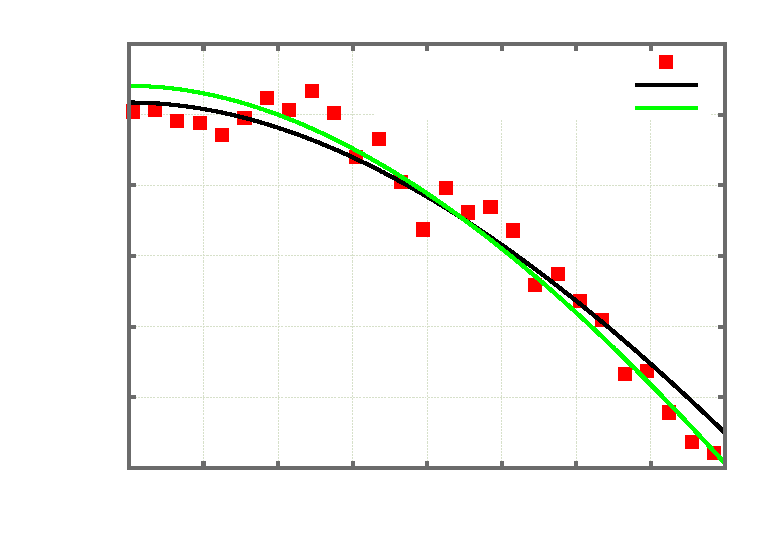
\includegraphics{pmfa_4xballs}}%
    \gplfronttext
  \end{picture}%
\endgroup
}
         \caption{Simulation performed with 200 balls (cf. \cref{fig:pmfa} with
         50 balls). Note the fluctuation behaviour as the depletion zones
         overlap.}
         \label{fig:4xballs}
      \end{minipage}~\hspace*{1em}
      \begin{minipage}[t]{.6\textwidth}		
         \vspace{0pt}
         \centering
         \resizebox{\columnwidth}{!}{% GNUPLOT: LaTeX picture with Postscript
\begingroup
  \makeatletter
  \providecommand\color[2][]{%
    \GenericError{(gnuplot) \space\space\space\@spaces}{%
      Package color not loaded in conjunction with
      terminal option `colourtext'%
    }{See the gnuplot documentation for explanation.%
    }{Either use 'blacktext' in gnuplot or load the package
      color.sty in LaTeX.}%
    \renewcommand\color[2][]{}%
  }%
  \providecommand\includegraphics[2][]{%
    \GenericError{(gnuplot) \space\space\space\@spaces}{%
      Package graphicx or graphics not loaded%
    }{See the gnuplot documentation for explanation.%
    }{The gnuplot epslatex terminal needs graphicx.sty or graphics.sty.}%
    \renewcommand\includegraphics[2][]{}%
  }%
  \providecommand\rotatebox[2]{#2}%
  \@ifundefined{ifGPcolor}{%
    \newif\ifGPcolor
    \GPcolortrue
  }{}%
  \@ifundefined{ifGPblacktext}{%
    \newif\ifGPblacktext
    \GPblacktexttrue
  }{}%
  % define a \g@addto@macro without @ in the name:
  \let\gplgaddtomacro\g@addto@macro
  % define empty templates for all commands taking text:
  \gdef\gplbacktext{}%
  \gdef\gplfronttext{}%
  \makeatother
  \ifGPblacktext
    % no textcolor at all
    \def\colorrgb#1{}%
    \def\colorgray#1{}%
  \else
    % gray or color?
    \ifGPcolor
      \def\colorrgb#1{\color[rgb]{#1}}%
      \def\colorgray#1{\color[gray]{#1}}%
      \expandafter\def\csname LTw\endcsname{\color{white}}%
      \expandafter\def\csname LTb\endcsname{\color{black}}%
      \expandafter\def\csname LTa\endcsname{\color{black}}%
      \expandafter\def\csname LT0\endcsname{\color[rgb]{1,0,0}}%
      \expandafter\def\csname LT1\endcsname{\color[rgb]{0,1,0}}%
      \expandafter\def\csname LT2\endcsname{\color[rgb]{0,0,1}}%
      \expandafter\def\csname LT3\endcsname{\color[rgb]{1,0,1}}%
      \expandafter\def\csname LT4\endcsname{\color[rgb]{0,1,1}}%
      \expandafter\def\csname LT5\endcsname{\color[rgb]{1,1,0}}%
      \expandafter\def\csname LT6\endcsname{\color[rgb]{0,0,0}}%
      \expandafter\def\csname LT7\endcsname{\color[rgb]{1,0.3,0}}%
      \expandafter\def\csname LT8\endcsname{\color[rgb]{0.5,0.5,0.5}}%
    \else
      % gray
      \def\colorrgb#1{\color{black}}%
      \def\colorgray#1{\color[gray]{#1}}%
      \expandafter\def\csname LTw\endcsname{\color{white}}%
      \expandafter\def\csname LTb\endcsname{\color{black}}%
      \expandafter\def\csname LTa\endcsname{\color{black}}%
      \expandafter\def\csname LT0\endcsname{\color{black}}%
      \expandafter\def\csname LT1\endcsname{\color{black}}%
      \expandafter\def\csname LT2\endcsname{\color{black}}%
      \expandafter\def\csname LT3\endcsname{\color{black}}%
      \expandafter\def\csname LT4\endcsname{\color{black}}%
      \expandafter\def\csname LT5\endcsname{\color{black}}%
      \expandafter\def\csname LT6\endcsname{\color{black}}%
      \expandafter\def\csname LT7\endcsname{\color{black}}%
      \expandafter\def\csname LT8\endcsname{\color{black}}%
    \fi
  \fi
  \setlength{\unitlength}{0.0500bp}%
  \begin{picture}(7200.00,5040.00)%
    \gplgaddtomacro\gplbacktext{%
      \colorrgb{0.42,0.42,0.42}%
      \put(946,704){\makebox(0,0)[r]{\strut{}-8}}%
      \colorrgb{0.42,0.42,0.42}%
      \put(946,1213){\makebox(0,0)[r]{\strut{}-7.5}}%
      \colorrgb{0.42,0.42,0.42}%
      \put(946,1722){\makebox(0,0)[r]{\strut{}-7}}%
      \colorrgb{0.42,0.42,0.42}%
      \put(946,2231){\makebox(0,0)[r]{\strut{}-6.5}}%
      \colorrgb{0.42,0.42,0.42}%
      \put(946,2740){\makebox(0,0)[r]{\strut{}-6}}%
      \colorrgb{0.42,0.42,0.42}%
      \put(946,3248){\makebox(0,0)[r]{\strut{}-5.5}}%
      \colorrgb{0.42,0.42,0.42}%
      \put(946,3757){\makebox(0,0)[r]{\strut{}-5}}%
      \colorrgb{0.42,0.42,0.42}%
      \put(946,4266){\makebox(0,0)[r]{\strut{}-4.5}}%
      \colorrgb{0.42,0.42,0.42}%
      \put(946,4775){\makebox(0,0)[r]{\strut{}-4}}%
      \colorrgb{0.42,0.42,0.42}%
      \put(1651,484){\makebox(0,0){\strut{} 6}}%
      \colorrgb{0.42,0.42,0.42}%
      \put(2796,484){\makebox(0,0){\strut{} 7}}%
      \colorrgb{0.42,0.42,0.42}%
      \put(3941,484){\makebox(0,0){\strut{} 8}}%
      \colorrgb{0.42,0.42,0.42}%
      \put(5086,484){\makebox(0,0){\strut{} 9}}%
      \colorrgb{0.42,0.42,0.42}%
      \put(6231,484){\makebox(0,0){\strut{} 10}}%
      \colorrgb{0.42,0.42,0.42}%
      \put(176,2739){\rotatebox{-270}{\makebox(0,0){\strut{}$-ln(H(r))+ln(r^2)$}}}%
      \colorrgb{0.42,0.42,0.42}%
      \put(3940,154){\makebox(0,0){\strut{}$r$}}%
      \colorrgb{0.42,0.42,0.42}%
      \put(3940,4665){\makebox(0,0){\strut{}}}%
    }%
    \gplgaddtomacro\gplfronttext{%
      \csname LTb\endcsname%
      \put(5804,4602){\makebox(0,0)[r]{\strut{}Simulation results}}%
      \csname LTb\endcsname%
      \put(5804,4382){\makebox(0,0)[r]{\strut{}$V_{big}$ omitted}}%
      \csname LTb\endcsname%
      \put(5804,4162){\makebox(0,0)[r]{\strut{}$V_{big}$ not omitted}}%
    }%
    \gplbacktext
    \put(0,0){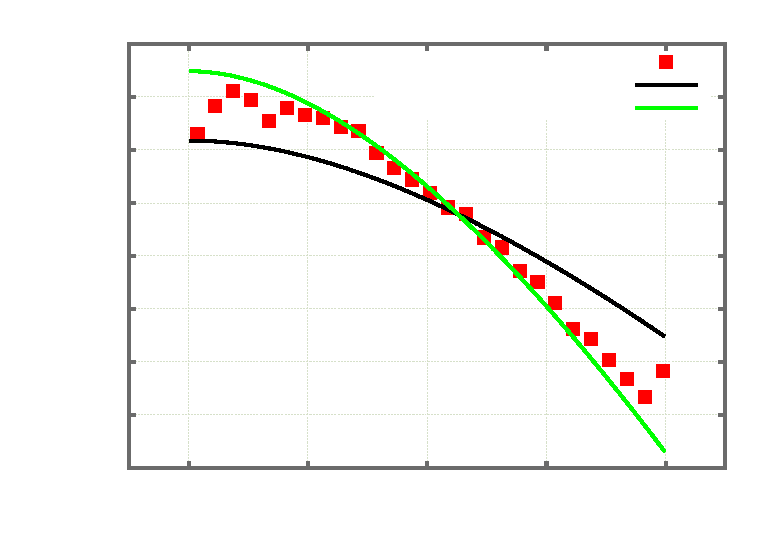
\includegraphics{pmfa_gigaball}}%
    \gplfronttext
  \end{picture}%
\endgroup
}
         \caption{Bigger ball here holds a radius of 20 length units (cf.
         \cref{fig:pmfa} with radius 12). Note the depletion zone limits being
         changed.} 
         \label{fig:gigaball}
      \end{minipage}
   \end{figure}

   The system does behave as expected, achieving a global minimum when the
   bigger ball is closer to the boundary. This simply is because of the fact
   that the smaller balls access a larger volume, and the system is thereby a
   subject to an increase in entropy.  

   \begin{figure}[H]
      \centering
      \resizebox{.6\columnwidth}{!}{% GNUPLOT: LaTeX picture with Postscript
\begingroup
  \makeatletter
  \providecommand\color[2][]{%
    \GenericError{(gnuplot) \space\space\space\@spaces}{%
      Package color not loaded in conjunction with
      terminal option `colourtext'%
    }{See the gnuplot documentation for explanation.%
    }{Either use 'blacktext' in gnuplot or load the package
      color.sty in LaTeX.}%
    \renewcommand\color[2][]{}%
  }%
  \providecommand\includegraphics[2][]{%
    \GenericError{(gnuplot) \space\space\space\@spaces}{%
      Package graphicx or graphics not loaded%
    }{See the gnuplot documentation for explanation.%
    }{The gnuplot epslatex terminal needs graphicx.sty or graphics.sty.}%
    \renewcommand\includegraphics[2][]{}%
  }%
  \providecommand\rotatebox[2]{#2}%
  \@ifundefined{ifGPcolor}{%
    \newif\ifGPcolor
    \GPcolortrue
  }{}%
  \@ifundefined{ifGPblacktext}{%
    \newif\ifGPblacktext
    \GPblacktexttrue
  }{}%
  % define a \g@addto@macro without @ in the name:
  \let\gplgaddtomacro\g@addto@macro
  % define empty templates for all commands taking text:
  \gdef\gplbacktext{}%
  \gdef\gplfronttext{}%
  \makeatother
  \ifGPblacktext
    % no textcolor at all
    \def\colorrgb#1{}%
    \def\colorgray#1{}%
  \else
    % gray or color?
    \ifGPcolor
      \def\colorrgb#1{\color[rgb]{#1}}%
      \def\colorgray#1{\color[gray]{#1}}%
      \expandafter\def\csname LTw\endcsname{\color{white}}%
      \expandafter\def\csname LTb\endcsname{\color{black}}%
      \expandafter\def\csname LTa\endcsname{\color{black}}%
      \expandafter\def\csname LT0\endcsname{\color[rgb]{1,0,0}}%
      \expandafter\def\csname LT1\endcsname{\color[rgb]{0,1,0}}%
      \expandafter\def\csname LT2\endcsname{\color[rgb]{0,0,1}}%
      \expandafter\def\csname LT3\endcsname{\color[rgb]{1,0,1}}%
      \expandafter\def\csname LT4\endcsname{\color[rgb]{0,1,1}}%
      \expandafter\def\csname LT5\endcsname{\color[rgb]{1,1,0}}%
      \expandafter\def\csname LT6\endcsname{\color[rgb]{0,0,0}}%
      \expandafter\def\csname LT7\endcsname{\color[rgb]{1,0.3,0}}%
      \expandafter\def\csname LT8\endcsname{\color[rgb]{0.5,0.5,0.5}}%
    \else
      % gray
      \def\colorrgb#1{\color{black}}%
      \def\colorgray#1{\color[gray]{#1}}%
      \expandafter\def\csname LTw\endcsname{\color{white}}%
      \expandafter\def\csname LTb\endcsname{\color{black}}%
      \expandafter\def\csname LTa\endcsname{\color{black}}%
      \expandafter\def\csname LT0\endcsname{\color{black}}%
      \expandafter\def\csname LT1\endcsname{\color{black}}%
      \expandafter\def\csname LT2\endcsname{\color{black}}%
      \expandafter\def\csname LT3\endcsname{\color{black}}%
      \expandafter\def\csname LT4\endcsname{\color{black}}%
      \expandafter\def\csname LT5\endcsname{\color{black}}%
      \expandafter\def\csname LT6\endcsname{\color{black}}%
      \expandafter\def\csname LT7\endcsname{\color{black}}%
      \expandafter\def\csname LT8\endcsname{\color{black}}%
    \fi
  \fi
  \setlength{\unitlength}{0.0500bp}%
  \begin{picture}(7200.00,5040.00)%
    \gplgaddtomacro\gplbacktext{%
      \colorrgb{0.42,0.42,0.42}%
      \put(814,704){\makebox(0,0)[r]{\strut{}-10}}%
      \colorrgb{0.42,0.42,0.42}%
      \put(814,1286){\makebox(0,0)[r]{\strut{}-9}}%
      \colorrgb{0.42,0.42,0.42}%
      \put(814,1867){\makebox(0,0)[r]{\strut{}-8}}%
      \colorrgb{0.42,0.42,0.42}%
      \put(814,2449){\makebox(0,0)[r]{\strut{}-7}}%
      \colorrgb{0.42,0.42,0.42}%
      \put(814,3030){\makebox(0,0)[r]{\strut{}-6}}%
      \colorrgb{0.42,0.42,0.42}%
      \put(814,3612){\makebox(0,0)[r]{\strut{}-5}}%
      \colorrgb{0.42,0.42,0.42}%
      \put(814,4193){\makebox(0,0)[r]{\strut{}-4}}%
      \colorrgb{0.42,0.42,0.42}%
      \put(814,4775){\makebox(0,0)[r]{\strut{}-3}}%
      \colorrgb{0.42,0.42,0.42}%
      \put(946,484){\makebox(0,0){\strut{} 0}}%
      \colorrgb{0.42,0.42,0.42}%
      \put(2011,484){\makebox(0,0){\strut{} 2}}%
      \colorrgb{0.42,0.42,0.42}%
      \put(3076,484){\makebox(0,0){\strut{} 4}}%
      \colorrgb{0.42,0.42,0.42}%
      \put(4141,484){\makebox(0,0){\strut{} 6}}%
      \colorrgb{0.42,0.42,0.42}%
      \put(5206,484){\makebox(0,0){\strut{} 8}}%
      \colorrgb{0.42,0.42,0.42}%
      \put(6271,484){\makebox(0,0){\strut{} 10}}%
      \colorrgb{0.42,0.42,0.42}%
      \put(176,2739){\rotatebox{-270}{\makebox(0,0){\strut{}$-ln(H(r))+ln(r^2)$}}}%
      \colorrgb{0.42,0.42,0.42}%
      \put(3874,154){\makebox(0,0){\strut{}$r$}}%
      \colorrgb{0.42,0.42,0.42}%
      \put(3874,4665){\makebox(0,0){\strut{}}}%
    }%
    \gplgaddtomacro\gplfronttext{%
    }%
    \gplbacktext
    \put(0,0){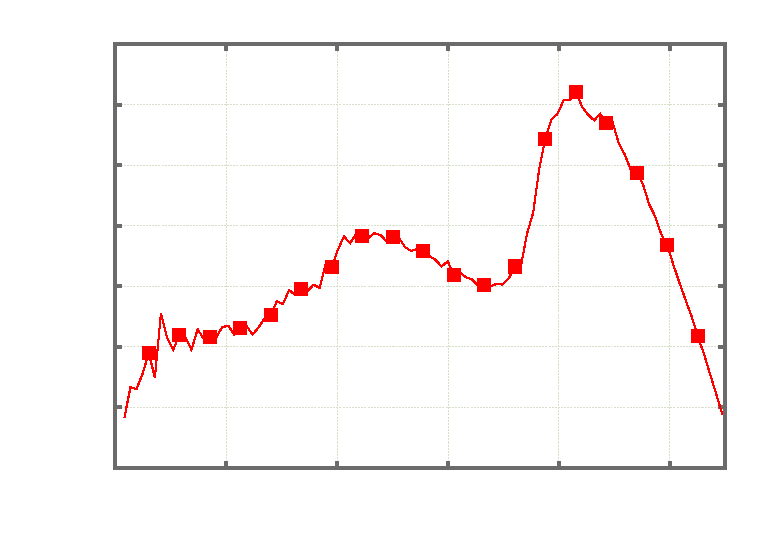
\includegraphics{exc2}}%
    \gplfronttext
  \end{picture}%
\endgroup
}
      \caption{Potential of mean force graph for a high-density system in two
         dimensions.
      Simulation settings are $R_s = 22, R = 11, r = 1.7$, and otherwise as
      previously stated.}
      \label{fig:exc2}            
   \end{figure}

   More clearly now in the denser system, minimas apart from the origin are
   present, most notably around the value of 7 length units in \cref{fig:exc2}.
   Because of the higher density, this is assumed to correspond to the smaller
   balls aligning up at the boundary, preventing the larger molecule from moving
   there, and thereby incapacitating the system somewhat. It ought also to be
   possible for the balls to assume a thicker layer directly around the larger
   ball, as can be imagined to
   happen in the region $<4$ length units, although sparse data makes the
   conclusion hard to make. It should be noted, however, that the successive
   decrease as can be seen in the region $r \rightarrow 0$ does not
   necessarily correspond to a factual decrease in free energy, but is instead
   the consequence of lack of data in this region. Nevertheless, it can
   certainly be imagined that the small balls might align so that the larger one
   is ``locked in'' in the center, and so the results might hold at least some
   significance, though further simulations are required to reveal the nature of
   this.

   The barrier between the first and the second minima ought however to
   correspond to the additional effort needed for the macromolecule to penetrate the
   layer of numerous smaller balls in order to reach the boundary.  

   Lastly, when the shape of the cavity is changed from a circular shape towards
   that of an ellipsis, other dynamics appear. Since data for the free energy is
   harder to quantify in this case, the dynamics can instead be understood by
   examining the real-time illustration of the macromolecule's positions during
   a simulation, provided in \cref{fig:exc3}.
   
   \begin{figure}[H]
      \centering
      \resizebox{.6\columnwidth}{!}{% GNUPLOT: LaTeX picture with Postscript
\begingroup
  \makeatletter
  \providecommand\color[2][]{%
    \GenericError{(gnuplot) \space\space\space\@spaces}{%
      Package color not loaded in conjunction with
      terminal option `colourtext'%
    }{See the gnuplot documentation for explanation.%
    }{Either use 'blacktext' in gnuplot or load the package
      color.sty in LaTeX.}%
    \renewcommand\color[2][]{}%
  }%
  \providecommand\includegraphics[2][]{%
    \GenericError{(gnuplot) \space\space\space\@spaces}{%
      Package graphicx or graphics not loaded%
    }{See the gnuplot documentation for explanation.%
    }{The gnuplot epslatex terminal needs graphicx.sty or graphics.sty.}%
    \renewcommand\includegraphics[2][]{}%
  }%
  \providecommand\rotatebox[2]{#2}%
  \@ifundefined{ifGPcolor}{%
    \newif\ifGPcolor
    \GPcolortrue
  }{}%
  \@ifundefined{ifGPblacktext}{%
    \newif\ifGPblacktext
    \GPblacktexttrue
  }{}%
  % define a \g@addto@macro without @ in the name:
  \let\gplgaddtomacro\g@addto@macro
  % define empty templates for all commands taking text:
  \gdef\gplbacktext{}%
  \gdef\gplfronttext{}%
  \makeatother
  \ifGPblacktext
    % no textcolor at all
    \def\colorrgb#1{}%
    \def\colorgray#1{}%
  \else
    % gray or color?
    \ifGPcolor
      \def\colorrgb#1{\color[rgb]{#1}}%
      \def\colorgray#1{\color[gray]{#1}}%
      \expandafter\def\csname LTw\endcsname{\color{white}}%
      \expandafter\def\csname LTb\endcsname{\color{black}}%
      \expandafter\def\csname LTa\endcsname{\color{black}}%
      \expandafter\def\csname LT0\endcsname{\color[rgb]{1,0,0}}%
      \expandafter\def\csname LT1\endcsname{\color[rgb]{0,1,0}}%
      \expandafter\def\csname LT2\endcsname{\color[rgb]{0,0,1}}%
      \expandafter\def\csname LT3\endcsname{\color[rgb]{1,0,1}}%
      \expandafter\def\csname LT4\endcsname{\color[rgb]{0,1,1}}%
      \expandafter\def\csname LT5\endcsname{\color[rgb]{1,1,0}}%
      \expandafter\def\csname LT6\endcsname{\color[rgb]{0,0,0}}%
      \expandafter\def\csname LT7\endcsname{\color[rgb]{1,0.3,0}}%
      \expandafter\def\csname LT8\endcsname{\color[rgb]{0.5,0.5,0.5}}%
    \else
      % gray
      \def\colorrgb#1{\color{black}}%
      \def\colorgray#1{\color[gray]{#1}}%
      \expandafter\def\csname LTw\endcsname{\color{white}}%
      \expandafter\def\csname LTb\endcsname{\color{black}}%
      \expandafter\def\csname LTa\endcsname{\color{black}}%
      \expandafter\def\csname LT0\endcsname{\color{black}}%
      \expandafter\def\csname LT1\endcsname{\color{black}}%
      \expandafter\def\csname LT2\endcsname{\color{black}}%
      \expandafter\def\csname LT3\endcsname{\color{black}}%
      \expandafter\def\csname LT4\endcsname{\color{black}}%
      \expandafter\def\csname LT5\endcsname{\color{black}}%
      \expandafter\def\csname LT6\endcsname{\color{black}}%
      \expandafter\def\csname LT7\endcsname{\color{black}}%
      \expandafter\def\csname LT8\endcsname{\color{black}}%
    \fi
  \fi
  \setlength{\unitlength}{0.0500bp}%
  \begin{picture}(7200.00,5040.00)%
    \gplgaddtomacro\gplbacktext{%
      \csname LTb\endcsname%
      \put(814,704){\makebox(0,0)[r]{\strut{}-40}}%
      \put(814,1213){\makebox(0,0)[r]{\strut{}-30}}%
      \put(814,1722){\makebox(0,0)[r]{\strut{}-20}}%
      \put(814,2231){\makebox(0,0)[r]{\strut{}-10}}%
      \put(814,2740){\makebox(0,0)[r]{\strut{} 0}}%
      \put(814,3248){\makebox(0,0)[r]{\strut{} 10}}%
      \put(814,3757){\makebox(0,0)[r]{\strut{} 20}}%
      \put(814,4266){\makebox(0,0)[r]{\strut{} 30}}%
      \put(814,4775){\makebox(0,0)[r]{\strut{} 40}}%
      \put(946,484){\makebox(0,0){\strut{}-80}}%
      \put(1678,484){\makebox(0,0){\strut{}-60}}%
      \put(2410,484){\makebox(0,0){\strut{}-40}}%
      \put(3142,484){\makebox(0,0){\strut{}-20}}%
      \put(3875,484){\makebox(0,0){\strut{} 0}}%
      \put(4607,484){\makebox(0,0){\strut{} 20}}%
      \put(5339,484){\makebox(0,0){\strut{} 40}}%
      \put(6071,484){\makebox(0,0){\strut{} 60}}%
      \put(6803,484){\makebox(0,0){\strut{} 80}}%
      \put(176,2739){\rotatebox{-270}{\makebox(0,0){\strut{}$\Delta y$}}}%
      \put(3874,154){\makebox(0,0){\strut{}$\Delta x$}}%
    }%
    \gplgaddtomacro\gplfronttext{%
    }%
    \gplbacktext
    \put(0,0){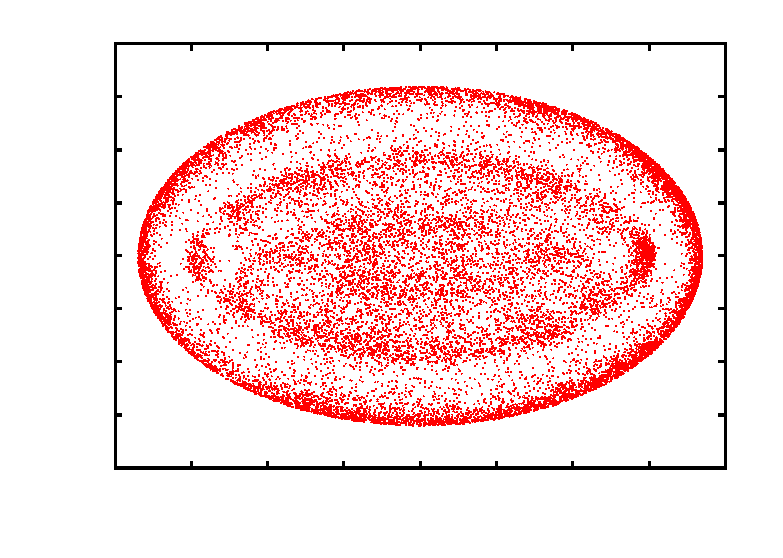
\includegraphics{exc3}}%
    \gplfronttext
  \end{picture}%
\endgroup
}
      \caption{Position of the larger molecule in a 2D-landscape within a 
      ellipsoidal cavity. The system is as in the previous example in a high-density 
      configuration, where the smaller balls make up a fraction of $\sim 30~\%$ of the
      available volume.}
      \label{fig:exc3}            
   \end{figure}

   Here the same behaviour which brought about the result with several minima
   in the previous simulation is come into display. Clearly, the larger ball has
   a direct bias towards some one--two boundaries within the cavity, as well as the
   outer rim. As in the previous simulation, this ought to be the result of many
   smaller balls layering up, so that the larger ball must pass through them in
   order to reach the outer boundary. Notably, in the ellipsoidal extremes where
   $\Delta y \approx 0$ the bias for the ball to be positioned there is stronger 
   than in other parts of the ellipsoidal boundary. This should correspond to
   the lack of available space to move within our two dimensions, so that the
   larger ball would to a higher extent be forced to move \emph{through} the
   small balls in order to shift its position markedly. The collisional forces
   from the small ball will therefore at those extremes further prevent the ball
   from moving than in other cases. Indeed, because the entropical forces will
   push the ball towards the positions where the area of the overlapping
   depletion zones will be maximized, the thinner parts of the ellipsis make a
   natural habitat for this phenomenon. The macromolecule simply \emph{fits}
   better into the edges where the zones overlap maximally.  

\section{Conclusions}
   Our results have shown that it is indeed possible to model depletionary
   forces through simple approximations and the concept of thermodynamics. In
   particular, it can be seen that a larger molecule in fact is pushed towards
   the boundaries of a system in correspondence with the concept of maximizing
   the overlapping depletion zones which forelie. 
   
   When the curvature of the
   boundary to a higher extent corresponds to the surface of the macromolecule,
   this is even more apparent, and the system will exhibit a corresponding
   behaviour to zones abiding to this property. 

   In practice, this can certainly be used in biological contexts to explain the
   gathering and interaction of similar-size or well-fitting proteins, and possibly 
   further, not here analyzed, extensions of this forcing phenomenon. 

\begin{thebibliography}{99}
   \bibitem{wine}
      Moreno, Juan; Peinado, Rafael, 
      \emph{Enological Chemistry}: 325-326,
      Elsevier Inc, 
      San Diego, 
      2012. 
   \bibitem{lecnotes}
      Anna Bille,
      \emph{Computer Assignment 1: Depletion forces},
      Lund University,
      2015.  
\end{thebibliography}
\end{document}

